\documentclass[11.5pt]{sig-alternate} % sets document style to sig-alternate
% packages
% typesetting
%\usepackage{dirtytalk} % typset quotations easier (\say{stuff})
\usepackage{hanging} % hanging paragraphs
\usepackage[defaultlines=3,all]{nowidow} % avoid widows
\usepackage[pdfpagelabels=false]{hyperref} % produce hypertext links, includes backref and nameref
\usepackage{xurl} % defines url linebreaks, loads url package
\usepackage{microtype}
%\usepackage[super]{nth} % easily create superscript ordinal numbers with \nth{x}
\usepackage{textcomp}
\newcommand{\texttildemid}{\raisebox{0.4ex}{\texttildelow}}
% layout
%\usepackage{enumitem} % control layout of itemize, enumerate, description
\usepackage{fancyhdr} % control page headers and footers
\usepackage{float} % improved interface for floating objects
%\usepackage{multicol} % intermix single and multiple column pages
% language
\usepackage[utf8]{inputenc} % accept different input encodings
\usepackage[english]{babel} % multilanguage support
% misc
\usepackage{graphicx} % builds upon graphics package, \includegraphics
%\usepackage{lastpage} % reference number of pages
%\usepackage{comment} % exclude portions of text (?)
\usepackage{xcolor} % color extensions
\usepackage[backend=biber, style=apa]{biblatex} % sophisticated bibliographies % necessary for HTML to display author info and date on abstract page
\usepackage{csquotes} % advanced quotations, makes biblatex happy
\usepackage{authblk} % support for footnote style author/affiliation
% tables and figures
\usepackage{tabularray}
\UseTblrLibrary{varwidth}
%\usepackage{array} % extend array and tabular environments
\usepackage{caption} % customize captions in figures and tables (rotating captions, sideways captions, etc)
%\usepackage{cuted} % allow mixing of \onecolumn and \twocolumn on same page
\usepackage{multirow} % create tabular cells spanning multiple rows
%\usepackage{subfigure} % deprecated, support for manipulation of small figures
%\usepackage{tabularx} % extension of tabular with column designator "x", creates paragraph-like column whose width automatically expands
%\usepackage{wrapfig} % allows figures or tables to have text wrapped around them
%\usepackage{booktabs} % better rules
% dummy text
%\usepackage{blindtext} % blind text dummy text
%\usepackage{kantlipsum} % Kant style dummy text
\usepackage{lipsum} %lorem ipsum dummy text
\usepackage{enumitem}
% other helpful packages may be booktabs, longtable, longtabu, microtype

\pagestyle{fancy} % sets pagestyle to fancy for fancy headers and footers

% header and footer
% modern way to set header image
\renewcommand{\headrulewidth}{0pt} % defines thickness of line under header
\renewcommand{\footrulewidth}{0pt} % defines thickness of line above header
\setlength\headheight{80.0pt} % sets height between top margin and header image, effectively moves page contents down
\addtolength{\textheight}{-80.0pt} % seems to affect the lower height. maybe only works properly if footer numbers enabled?
\fancyhf{}
\fancyhead[CE, CO]{
\includegraphics[width=\textwidth]{headerImage.png}}
% footer
%\fancyfoot[LE,LO]{Article Title Here \\ DOI: }% left footer article title and doi
%\fancyfoot[CE,CO]{{}} % center footer empty
%\fancyfoot[RE,RO]{\thepage} % right footer page numbers
%\pagenumbering{arabic} % arabic (1, 2, 3) numbering in footer

\hypersetup{colorlinks=true,urlcolor=blue} % sets link color to blue
\urlstyle{same} % sets url typeface to same as rest of text

% set caption and figure to italics, label bold, left align captions, does not transfer to HTML
\captionsetup{labelfont=bf, font={large, it}, justification=raggedright, singlelinecheck=false}
\renewcommand\theContinuedFloat{\alph{ContinuedFloat}}

%this next bit is confusing, but essentially changes the width of the abstract. Seems to have been copied from this https://tex.stackexchange.com/questions/151583/how-to-adjust-the-width-of-abstract
\let\oldabstract\abstract
\let\oldendabstract\endabstract
\makeatletter %changes @ catcode to enable modification (in parsep)
\renewenvironment{abstract} %alters the abstract environment
{\renewenvironment{quotation}%
               {\list{}{\addtolength{\leftmargin}{1em} % change this value to add or remove length to the the default ?
                        \listparindent 1.5em%
                        \itemindent    \listparindent%
                        \rightmargin   \leftmargin%
                        \parsep        \z@ \@plus\p@}%
                \item\relax}%
               {\endlist}%
\oldabstract}
{\oldendabstract}
\makeatother %changes @ catcode to disable modification

% checks
% italics -
% links -
% dashes - 
% tildes -
% dollars -
\begin{document}

\title{A Tale of Two Courses: Exploring Teacher Candidates’ Translation of Science and Special Education Methods Instruction Into Inclusive Science Practices}

\author[1]{\large \color{blue}Sami Kahn}
\author[1]{\large \color{blue}Ryan Pigman}
\author[1]{\large \color{blue}Jennifer Ottley}

\affil[1]{Ohio University}

\toappear{}
%% ABSTRACT
\maketitle
\begin{@twocolumnfalse} 
\begin{abstract}
\item 
\textit{Early childhood educators teach science to all students, including students with disabilities. Strategies for accommodating students with disabilities in science, including familiarity with equitable frameworks such as Universal Design for Learning (UDL) are therefore a critical aspect of early childhood teacher candidates’ pedagogical content knowledge (PCK). Such strategies are often emphasized in special education courses that are offered separately from science methods courses. This practice assumes that teacher candidates can synthesize and transfer those practices into their science lesson planning. To explore how teacher candidates actually assimilate the instruction on inclusive science that is taught in their preparation coursework, this study examined the early and late semester science lesson plans of 26 early childhood teacher candidates who were concurrently enrolled in science and special education methods courses. Qualitative and discourse analysis illuminated the following key findings: 1) Teacher candidates demonstrate a strong tendency to accommodate students with disabilities by having them rely on others both before and after extensive instruction; 2) Instruction appears to reduce teacher candidates’ accommodating students with disabilities through separate materials/activities/directions; 3) Principles of UDL were more evident in late semester lesson plans; and 4) Late semester lesson plans contained more “behavior oriented” language and concerns. These findings are discussed with particular attention paid to ways in which science and special education teacher educators might intervene at key junctures in teacher candidates’ lesson planning processes to promote student autonomy, science inquiry, and greater use of the continuum of adaptations that are available to them.}
\\ \\
Keywords: Inclusive Science, Teacher Preparation, Universal Design for Learning, Pedagogical Content Knowledge
\end{abstract}
\end{@twocolumnfalse}

%% AUTHOR INFORMATION

\textbf{*Corresponding Author, Sami Kahn}\\
\href{mailto: kahns@ohio.edu }{(kahns@ohio.edu)} \\
\textit{Submitted  Oct 10 2017 }\\
\textit{Accepted Nov 26 2017} \\
\textit{Published online Jan 3 2018} \\
\textit{DOI:10.14448/jsesd.08.0004} \\
\pagebreak
\clearpage
\begin{large}
\section*{INTRODUCTION}
How do science teacher candidates make sense of the instruction that they receive on inclusive practices in their methods courses? This is arguably a critical question given the strong emphasis on “science for all” in contemporary educational reform documents.  The National Science Teacher Association’s Pre-Service Science Teacher standards (NSTA, 2012) charge teacher preparation programs with ensuring that their graduates develop learning environments, lesson plans, and assessments that promote science literacy for all students. Similarly, the \textit{Next Generation Science Standards} [\textit{NGSS}] advance a comprehensive vision of inclusive science for all underrepresented groups in its section entitled, “All Standards, All Students” (NGSS Lead States, Appendix D, 2013). Yet despite consistent calls for preparation of science teachers to meet the needs of all students, science teachers are underprepared to teach students with disabilities in their classrooms (Irving, Nti, \& Johnson, 2007).  The lack of pre-service preparation in this area was punctuated in a recent survey of over 1000 science teachers, which found that informal, “on the job training” was cited as the primary source for inclusive science pedagogy (Kahn \& Lewis, 2014). This situation creates a pedagogical and arguably, a moral dilemma of placing new teachers in classrooms without ample preparation, a set-up for attitudinal and practical barriers. It is therefore not surprising that students with disabilities underperform on standardized science assessments and are underrepresented in science fields (National Assessment of Educational Progress [NAEP], National Center for Education Statistics [NCES], 2011; National Science Foundation [NSF], 2013).  

Science teacher preparation programs have a unique opportunity to capitalize on a recent bloom of research that examines inclusive science education from an array of paradigms (Mc\-Ginnis \& Kahn, 2014).  Yet a review of the literature exposes the lack of studies that examine how teacher candidates actually assimilate the instruction on inclusive science that is taught in their preparation coursework. To address this gap, we examined the early and late semester science lesson plans of 26 early childhood teacher candidates in light of the instruction they received in both their science and special education methods courses during the second semester of their junior year.   We used qualitative and discourse analysis to answer the following research questions (RQs): 

\begin{quote}
RQ1 – How do early childhood candidates articulate adaptations for students with disabilities in science lesson plans?

RQ2 – What is the impact of instruction on early childhood candidates’ number and quality of adaptations for students with disabilities in science lesson plans?
\end{quote}

To advance these questions, we position this research within a theoretical framework of inclusive science practices and pedagogical content knowledge. \\

\section*{THEORETICAL CONTEXT}

\subsection*{Approaches to Inclusive Science}

Approaches to science education for students with disabilities reflect a combination of cognitive, behavioral, and developmental perspectives each contributing varying visions for the more than six million students with disabilities in U.S. schools (National Center for Education Statistics, 2017). A glance at the history of inclusive science in the U.S. is helpful in situating the present study within research and practice contexts. 
	
Prior to the Education for All Handicapped Children Act (1975), passed by the U.S. Congress as PL94–142 and amended and renamed in 1990 as the Individuals with Disabilities Education Act (IDEA), students with disabilities were frequently educated in separate schools or classrooms, with science often viewed as an unnecessary facet of their education.  Science education in the special education classroom often emphasized explicit or direct teaching (Steele, 2005). With the advent of the IDEA’s mandate of a free appropriate public education in the least restrictive environment, students with disabilities were increasingly educated in general education classrooms, including science classrooms.  Inclusion focused on identifying adaptations in the delivery of, engagement with, and assessment of science in order to make it accessible for all students.  Adaptations that maintain performance expectations but simply “level the playing field” for students, such as enlarged print, audible thermometers, providing graphic organizers, or pre-teaching important concepts, are referred to as “accommodations.”  Adaptations that change the performance expectation, such as reducing the number of questions on a test or the number or scope of learning objectives, are referred to as “modifications.”  As the intent of the IDEA was for students’ educations to be individualized to meet their specific needs, an annual Individualized Education Program (IEP) was created for each student, which frequently mandated specific supports in science, such as modified equipment, extended time for testing, time with an intervention specialist to focus on science content, and so on.

A significant body of literature supports hands-on, inquiry-based science teaching with adaptations for students with a range of disabilities including learning disabilities (Taylor et al., 2012), physical and sensory disabilities (Wild \& Trundle, 2010), emotional disabilities (McCarthy, 2005), and intellectual disabilities (Miller, 2012).  While developing adaptations for specific students continues to be the most prevalent approach, a more critical approach to inclusive science education has emerged, one that questions disability as a social construct and identifies society rather than the student as the entity in need of remediation (Baglieri, Valle, Connor, \& Gallagher, 2011).  This notion of ability reflects a social model that promotes the development of physical, pedagogical, and attitudinal environments that support the success of all students in science (McGinnis \& Kahn, 2014).  Pedagogical frameworks such as Universal Design for Learning [UDL] (Meyer, Rose, \& Gordon, 2014) assume competence and require teachers to develop lessons and environments that provide flexibility in the way all students are engaged, in the way information is presented, and in the way students demonstrate learning. In addition, teachers utilizing UDL reduce barriers proactively for all students during lesson planning rather than adding in accommodations retroactively for individual students in order to maximize student access and participation. This approach has gained influence in both science and special education teacher preparation, particularly since UDL was recently defined and endorsed as a research-based approach to teaching all learners in the Every Student Succeeds Act (ESSA) of 2015 and the National Education Technology Plan (NETP, 2016).

Although a range of approaches are available to pre-service science teachers, research suggests that very little instruction specific to students with disabilities in science is included in teacher education programs.  The majority of teacher education programs rely on a single course in special education to address the specific adaptations needed for various content foci (Cameron \& Cook, 2007; Government Accountability Office, 2009). This leads teachers in the field to note that their first consideration of students with disabilities is when they actually teach them in their classrooms, which may lead to feelings of frustration, inadequacy, and resentment (Kahn \& Lewis, 2014). Sadly, lack of preparation may overshadow the fact that most science teachers hold positive perspectives in regard to inclusion, at least in theory (McGinnis, 2000), as they recognize the intellectual, practical, and social benefits of rigorous science classes for students with disabilities (Mastropieri, et al., 1998).  Supporting science teacher candidates’ understanding of a range of inclusive science strategies is critical to supporting science opportunities for all students. 

\subsection*{Putting Theory Into Practice: Pedagogical Content Knowledge (PCK)}

An assumption underlying teacher preparation is that pre-service teacher candidates are able to assimilate the strategies that they learn in their theory and methods courses into actual practice (Grossman, Hammerness, \& McDonald, 2009).  Instruction on the theories and practices for ensuring access for all students is part and parcel of the pedagogical content knowledge [PCK] (Shulman, 1986) that is critical for successful inclusive science teaching.  PCK is defined here as “the knowledge that a teacher uses to provide teaching situations that help learners make sense of particular science content” (Loughran, Milroy, Berry, Gunstone, \& Mulhall, 2001, p. 289). Although models of PCK vary, many involve consideration of teachers’ knowledge of subject matter, pedagogical strategies, and their students.  Enactment of inclusive science strategies would therefore necessitate knowledge of how students with disabilities learn and what strategies would likely be successful. Lesson plans can serve as a critical indicator of teacher candidates’ PCK (Kellner, Gullberg, Attorps, Thorén, \& Tärneberg, 2011) as they represent teacher candidates’ articulation of the strategies that are appropriate for addressing the learning needs of the students they encounter in their classroom placements, including students with disabilities. We hypothesized that teacher candidates’ lesson plans later in the semester would reflect richer use of inclusive science strategies, including UDL tenets, and more meaningful adaptations after having received instruction in their courses and having had greater time in their teaching field placements, as both of these inputs would presumably contribute to PCK.

\section*{METHODOLOGY}

\subsection*{Study Context}

Our College of Education, which is located in a rural setting in the Midwest U.S., serves approximately 1600 undergraduate and 900 graduate students. We use a clinical model for teacher preparation, thus ensuring extensive in-school opportunities for teacher candidates beginning in their sophomore year and benefitting from close relationships with partner schools (National Council for Accreditation of Teacher Education, 2010). For this study, 26 early childhood candidates voluntarily participated by allowing examination of the lesson plans they developed for their science methods course entitled, “Teaching Science in Early Childhood,” which is offered within our Department of Teacher Education. This course is taught in the spring semester of their junior year, and is taken concurrently with a course on adaptations offered within the same department. The adaptations course is the only required course specifically focused on inclusive pedagogy in the early childhood program. 

\subsection*{The Courses}

All 26 teacher candidates took both the science methods course and a course entitled, “Instructional Adaptations for Early Childhood Learners with Exceptionalities and Diverse Needs,” which was taught by special education faculty within the same Department of Teacher Education.  Excerpts from the course descriptions are as follows: 

Excerpt from Early Childhood Science Methods Course Description: 

\begin{quote}
This course will combine pedagogical strategies, science content and process skills, as well the philosophical and historical underpinnings of constructivist elementary science teaching and learning… to help you develop and implement meaningful science inquiry  lessons for all early childhood students… 
\end{quote}

Excerpt from Adaptations Course Description:

\begin{quote}
The course content includes universally designed instruction, individually designed instruction, curriculum modifications, instructional and management adaptations, effective collaboration strategies, accessing related and support services, and skills required for managing and instructing an inclusive early childhood classroom… 
\end{quote}

The science methods course included instruction on specific adaptations for students with disabilities and on UDL during week five and then continuously throughout the remainder of the course.  The special education adaptations course also began discussions of adaptations in week five and continued with a range of approaches to support students’ social, emotional, and physical needs.  We report the course outlines, presented in parallel in Table 1.  

\begin{table*}[htbp]
\caption{Science and Special Education Methods Course Topics By Week}
\begin{tabular}{|l|c|l|}
\hline
\textbf{Science Methods Course Topics} & \textbf{Week \#} & \textbf{Special Education Methods Course Topics} \\ \hline
\begin{itemize}[noitemsep, topsep=0pt]
    \item Science as Inquiry
    \item Nature of Science (NOS)
    \item 5E Instructional Framework
    \item Science Standards
\end{itemize} & 1 & \begin{itemize}[noitemsep, topsep=0pt]
    \item Review of Course Materials
    \item Overview of Key Terms
    \item Introduction to ECSE
    \item Person-First Language
\end{itemize} \\ \hline
\textit{No Class--MLK} & 2 & \begin{itemize}[noitemsep, topsep=0pt]
    \item Educating Young Children with Special Needs: The Challenge
\end{itemize} \\ \hline
\begin{itemize}[noitemsep, topsep=0pt]
    \item NOS, continued
    \item Science Safety
    \item Identifying Misconceptions
\end{itemize} & 3 & \begin{itemize}[noitemsep, topsep=0pt]
    \item Referral Process
    \item Developing Individualized Intervention Plans and Programs
    \item Monitoring Progress
\end{itemize} \\ \hline
\begin{itemize}[noitemsep, topsep=0pt]
    \item Identifying Misconceptions, Part 2
    \item Integration of Children’s Literature
\end{itemize}
\textbf{--5E Lesson Plan Due--} & 4 & \begin{itemize}[noitemsep, topsep=0pt]
    \item Designing Instructional Programs
\end{itemize} \\ \hline
\begin{itemize}[noitemsep, topsep=0pt]
    \item Science for All!
    \item Universal Design for Learning
    \item Differentiated Instruction
\end{itemize} & 5 & \begin{itemize}[noitemsep, topsep=0pt]
    \item Adaptation Continuum
\end{itemize} \\ \hline
\begin{itemize}[noitemsep, topsep=0pt]
    \item Cooperative Learning
    \item Integration of Math, Social Studies, and Technology
\end{itemize} & 6 & \begin{itemize}[noitemsep, topsep=0pt]
\item Positive Behavior Intervention and Supports
\item Promoting Emotional and Social Development
\end{itemize} \\ \hline
\begin{itemize}[noitemsep, topsep=0pt]
    \item Use of Instruments in Science
    \item Measurement with Young Students
    \item UDL Lesson Analysis Due
\end{itemize} & 7 & \begin{itemize}[noitemsep, topsep=0pt]
    \item Considerations for Teaching Children with Specific Disabilities
\end{itemize} \\ \hline
\begin{itemize}[noitemsep, topsep=0pt]
    \item Family Involvement in Science
    \item Teach Day Check-In
\end{itemize} & 8 & \begin{itemize}[noitemsep, topsep=0pt]
    \item Encouraging the Development of Cognitive Skills and Literacy
\end{itemize} \\ \hline
\textit{Spring Break} & 9 & \textit{Spring Break} \\ \hline
\begin{itemize}[noitemsep, topsep=0pt]
    \item Science Graphic Organizers
    \item Experimental Design
\end{itemize} \textbf{--Teach Day Lesson Plan Due--} & 10 & \begin{itemize}[noitemsep, topsep=0pt]
    \item Strengthening Motor and Self-Help Skills
\end{itemize} \\ \hline
\begin{itemize}[noitemsep, topsep=0pt]
    \item Outdoor Learning
    \item Citizen Science
\end{itemize} & 11 & \begin{itemize}[noitemsep, topsep=0pt]
    \item Nurturing Communication Skills
\end{itemize} \\ \hline
\begin{itemize}[noitemsep, topsep=0pt]
    \item Writing for Science
    \item Scaffolding Inquiry
\end{itemize} & 12 & \begin{itemize}[noitemsep, topsep=0pt]
    \item Teaming: Collaboration, Problem Solving, \& Inclusion Support
\end{itemize} \\ \hline
\begin{itemize}[noitemsep, topsep=0pt]
    \item Reading Comprehension Strategies in Science
    \item Argumentation in Science
\end{itemize} & 13 & \begin{itemize}[noitemsep, topsep=0pt]
    \item In Partnerships with Families
\end{itemize} \\ \hline
Student Presentations and Units & 14 & \begin{itemize}[noitemsep, topsep=0pt]
    \item Transitions in Early Childhood
    \item Home Visiting
\end{itemize} \\ \hline
Student Presentations and Units & 15 & Project-Based Learning Presentation \& Discussion \\ \hline
\end{tabular}
\end{table*}

\subsection*{The Lesson Plan Assignments}

The early childhood science methods course requirements included two lesson plan assignments that were the focus of the present research.  The “early” 5E Lesson Plan was due during week 4, prior to any explicit instruction on accommodating students with disabilities had been provided in either course. The “late” Teach Day Lesson Plan was due week 10, after four weeks of instruction on adaptations.  The “early” 5E Lesson Plans provided us with a pre-intervention baseline understanding of our students’ knowledge and articulation of inclusive science strategies.  We were then able to compare the findings from our analysis of the “early” 5E Lesson Plans with post-intervention “late” Teach Day Lesson Plans.  

\subsubsection*{5E Lesson Plan}
The first lesson plan assignment, which the science instructor assigned during the second week of the course, asked candidates to develop a science lesson plan for any K-3 grade using the BSCS 5E Instructional Model (Bybee, et al., 2006).  The instructor provided candidates with a lesson plan template that included lesson objectives, state and national standards, assessment plans, learning trajectories, materials, safety, and a section that required detailed instructions and rationales for teacher actions, as well as reflections on the teaching process.  The template included the steps in the 5E model in the teaching instructions section, which include, “Engage,” “Explore,” “Explain,” “Elaborate,” and “Evaluate.”  Finally, the template included a section entitled “Adaptations for Students with Special Needs.” This assignment was due during the fourth week of the class.

\subsubsection*{Teach Day Lesson Plan}
The second lesson plan assignment, which was assigned during the sixth week of the science methods course, asked teacher candidates to develop and teach one 5E inquiry lesson on their Teach Day (i.e., a day in which candidates were responsible for delivering all instruction in their classrooms). The lesson plan needed to engage children in collecting data and developing evidence-based explanations. The lesson, which was due during the tenth week of the course, was taught in their field placement classrooms during weeks eleven or twelve.  The template for this lesson plan was identical to the one provided for the “Early” 5E lesson assignment. 

\subsection*{The Researchers}

As the researcher is the instrument in qualitative analyses (Patton, 2002), we provide the reader with a brief overview of the researchers’ backgrounds. The first author of the study is a faculty member with expertise in science education who ascribes to a constructivist teaching philosophy with a strong social action bent.  The second author is a doctoral student in special education with several years of experience as a K-12 intervention specialist and interests in high-leverage practices and UDL. The third author is a faculty member with expertise in the education of young students with disabilities who holds a balanced view of the education such that some instruction should be child-led paired with other instruction that is teacher-led. All three researchers interpret “inclusion” in a broad sense, referring not simply to where a student is educated, but rather, to ensuring full access to high-quality science education.  We recognize that our differences is training colors our interpretations of the data; to address this, we took several steps, as described below, to enhance the trustworthiness (Lincoln \& Guba, 1985) of our study. 

\subsection*{Data Analysis}

Inductive thematic analysis of the lesson plans was done in three stages: (a) organizing and familiarizing, (b) coding and reducing (utilizing the constant comparative method), and (c) interpreting and representing (Ary, Jacobs, \& Sorenson, 2010). The data was coded manually using a parallel process whereby the first two authors began their analyses independently, then compared and refined findings, and then returned to the data independently over several iterations to ensure agreement and consistency. Keywords and phrases were highlighted and codes were developed.  Based on co-occurring codes, we consolidated codes into broader themes.  One area of particular difficulty (analytically speaking) was the question of coding for “Modified Objectives.”  It was not uncommon for teacher candidates to alter expectations by replacing writing with drawing or speaking, or for example, in the case of a classification activity, providing pre-determined categories for the students rather than having them generate categories themselves. In order to distinguish between simplifying, providing alternative means of expression, and “doing for” them, we looked at the objectives of the lesson.  If the adaptation impacted the lesson objectives in any way, we coded for “Modified Objectives.” If the adaptation did not impact the lesson objectives, but rather, provided alternative means of expression for the entire class, we coded for “UDL,” and if the adaptation had someone else doing a task for students with disabilities in any aspect of the activity that did not change lesson objectives, we coded for “Rely on Others.” We implemented analyst triangulation (Patton, 2002) by randomly selecting ten quotes from the data and sending them to the third author, who was asked to categorize the quotes within the themes in a manner that made sense to them. One discrepancy was noted relating to the abovementioned challenge; however, once the third author was provided with the lesson objectives for the quote, they revised their coding, which led to full agreement. No discrepancies were noted in any other of the categorizations, thus yielding high inter-rater reliability (Miles \& Huberman, 1994).  We also maintained an audit trail (Lincoln \& Guba, 1985) to bolster confirmability. We utilized discourse analysis to quantify the frequency of the codes. 

\section*{RESULTS}

The results of our analyses are presented in Tables 2 and 3 below.  Table 2 describes the “early” lesson plans, which preceded any instruction on specific adaptations from either the science or special education methods courses, listed in order of frequency. Table 3 describes the “late” lesson plans for the teacher candidates’ “Teach Day,” which followed instruction on adaptations and UDL in both the science and special education methods courses, also listed according to frequency.

\begin{table*}[htpb]
\caption{Early Semester (5E) Lesson Plan Themes and Frequencies}
\begin{tabular}{llc}
\hline
\textbf{Early (5E) Lesson Plan Theme} & \SetCell{c} \textbf{Theme Exemplars} & \textbf{Frequency} \\ \hline
Rely on Others & \begin{tabular}[x]{@{}l@{}} “If the students are not able to write what they want to record, I will pair them up with another student who they work well with and could help them write down.” \\ “I could also team them up with a buddy who could explain things and help them do the activity.” \end{tabular} & 20 \\
Use Separate Materials, Activities, Directions & \begin{tabular}[x]{@{}l@{}} “To adapt this experiment for children with special needs the teacher could pre-make the flubber for them so they do not have to do it themselves.” \\ “Have students use pencil and paper instead of cookies.” \end{tabular} & 19 \\
No Lesson Changes & \begin{tabular}[x]{@{}l@{}} “Photos are clear and in black and white so no child who has a visual impairment will feel unable to complete the assignment.” \\ “I will be reading the book to everyone so that students that are not strong readers will be able to focus on listening to the story and not trying to read the book.” \end{tabular} & 9 \\
Modify Objectives & \begin{tabular}[x]{@{}l@{}} “Pre-determined categories for the animal locomotion will be available.” \\ “Instead of writing in their journal they could tell me what they have learned.” \end{tabular} & 8 \\
UDL & “Pictures and words will be on the record sheet for students who may struggle with English or reading.” & 5 \\
\end{tabular}
\end{table*}

\begin{table*}[htpb]
\caption{Late Semester (Teach Day) Lesson Plan Themes and Frequencies}
\begin{tabular}{llc}
\hline
\textbf{Late Lesson Plan Theme} & \textbf{Theme Exemplar} & \textbf{Frequency} \\ \hline
Rely on Others & \begin{tabular}[x]{@{}l@{}} “If the students are not able to write what they want to record or the sentence about their roller coaster, I will pair them up with another student who they work well with and could help them write down what they are wanting to say.” \\ “If the student was in need of more support with this activity, they will be placed with a partner who is strong academically. Teacher will be there to offer support and ask reflective questions to be sure the student understands the concepts at hand.” \end{tabular} & 23 \\
UDL & \begin{tabular}[x]{@{}l@{}} “The experiment includes visuals, hands-on experiences, writing, and drawing. One of these forms could identify with a student more than the other forms.” \\ “Multiple means of representation were in place allowing students to hear instructions verbally, written, and with pictures.” \end{tabular} & 16 \\
Behavior-focused Adaptations & \begin{tabular}[x]{@{}l@{}} “Students who struggle with behavior will be given visual and verbal cues to remind them of the expected behaviors.” \\ “Positive reinforcing language will be in place to motivate students to show the expected behaviors.” \\ “He will be placed at a table to work at with specific students who are well behaved and do not follow his behavior when it is not correct.” \end{tabular} & 7 \\
Modify Objectives & “Instead of building the actual car, students can design blue prints. This takes away the testing aspect, but allows for students with sensorimotor restrictions to participate and share ideas as well.” & 6 \\
Use Separate Materials, Activities, Directions & \begin{tabular}[x]{@{}l@{}} “Students with sensory difficulties can be given different materials in order for them to still participate in the sorting” \\“Pre-make oobleck for them to explore with, without having to make it themselves (stirring the oobleck can be difficult as it gets hard very quickly).” \end{tabular} & 6 \\
No Lesson Changes & “The students are working in small groups, which will help bounce ideas off of each other and help them have a better understanding.” & 1 \\

\end{tabular}
\end{table*}
From these results, we have identified the following four key findings:
	
\begin{enumerate}[nosep]
    \item Both the “Early” and  “Late” lesson plans reflect a strong tendency on the part of the teacher candidates to accommodate students with disabilities by relying on others;
    \item The “Late” Teach Day Lesson plans reflect less tendency on the part of the teacher candidates to accommodate by using separate materials/activities/directions;
    \item The “Late” Teach Day Lesson plans contain more adaptations associated with UDL;
    \item The “Late” Teach Day Lesson plans contain more “behavior oriented” language and concerns.
\end{enumerate}
           
As we progressed through our coding, we began to notice that our themes were suggestive of a series of alternatives lending themselves to “versus coding” (Saldaña, 2016).  These themes indicated a spectrum of adaptations from which teacher candidates appeared to select at the extremes.  For example, teacher candidates chose either “relying on others” or “working alone” as diametrically opposed solutions to similar challenges.  We present our “versus codes” in Figure 1 below, followed by its implications in the Discussion section.  
 
\begin{figure}[h]
    \centering
    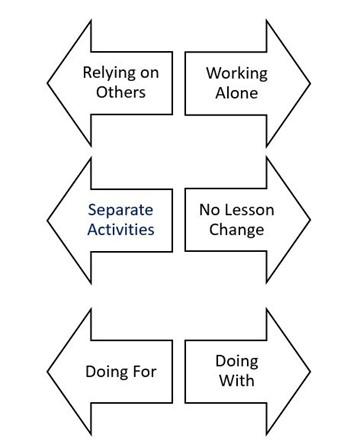
\includegraphics[width=0.7\linewidth]{images/fig1.jpg}
    \caption{ Versus coding scheme (Saldaña, 2016) emerging from lesson plan analysis}
\end{figure}

\section*{DISCUSSION}

Teacher candidates in this study utilized relying on others, rather than developing supports and environments that encourage autonomy, as the primary adaptation for students with disabilities, a finding in concert with prior research (McGinnis, 2003).  The fact that this adaptation was so prominent both before and after extensive instruction on a variety of adaptations implies that there are somewhat intractable barriers to the transfer of adaptations to science lesson planning.  We think that our “versus coding” framework (Figure 1) may provide some insight into teacher candidates’ thinking on this matter. Teacher candidates appeared to select between somewhat extreme ends of an adaptation continuum rather than exploring the “grey” areas that arguably represent the larger body of available adaptations that lay the path between inclusion and exclusion. When teacher candidates mentioned “working alone,” for example, their conception seemed to be one that was somewhat punitive rather than promoting autonomy.  Teacher candidates mentioned this adaptation as a response to misbehavior rather than as a product of scaffolding independence. Similarly, in both “early” and “late” lesson plans, teacher candidates who determined that separate activities or materials were necessary seemed to do so without considering or ruling out less extreme alternatives that could support full participation in the planned activity.

We felt it was particularly important to interrogate the decision to have students with disabilities rely on others as an adaptation since whether the reliance can be characterized as  “doing for” vs. “doing with” has profound implications for inquiry-based science.  If teachers (and teacher candidates) and peers “do for” their students (e.g., pre-cut materials, act as scribes, complete the hands-on aspects of the investigation, etc…), students have fewer opportunities to gain autonomy and develop the skills needed to progress in science.  For example, in one teacher candidate’s “early” lesson plan on the phases of the moon, the candidate’s instructions for the class involved modeling the phases by scraping varying amounts of cream from inside Oreo cookies to create half, quarter, and new moons.  However, for students with disabilities, the candidate offered the adaptation of “hav[ing] the cookies premade into different phases” (Code: “Doing for” – Teacher).  Clearly, this reliance on the teacher to essentially do the activity changes the objectives of the lesson and curbs any opportunity for the student to practice modeling skills. Likewise, another candidate offered that, during a lesson on floating and sinking, a student with visual impairments “can have another student or teacher verbally tell the student what the objects are and describe to them what happens when it is placed in water” (Code: “Doing for” – Students). The assumption that a student with a visual impairment can only passively stand by and have others place objects in water diminishes any opportunity for such a student to experience what it means for an object to float or sink (which they could presumably do by simply putting their hands in the water and feeling the positions of the objects) and to participate in the inquiry in any meaningful way.

Scaffolding autonomy, particularly in the context of inquiry is a critical practice in science for students with disabilities (Kahn, Feldman, \& Cooke, 2014). While autonomy was not originally a focus of our present study, our findings suggesting that teacher candidates hold strong inclinations toward accommodating students with disabilities by relying on others prompted us to develop a resource for teacher educators. From our findings, we were able to devise a decision tree (shown in Figure 2) that can inform science and special education teacher educators where they might intervene to guide teacher candidates to maximize positive social supports that encourage full participation of all students. For example, as it was a common adaptation for our candidates to suggest pairing students with disabilities with academically stronger students, science teacher educators can suggest that whole class peer tutoring (Scruggs \& Mastropieri, 2007; Therrien, et al, 2011) can accomplish the goal of having students learn from each other, but do so with all students sharing their expertise and no students being singled out as needing special assistance.  Similarly, suggesting the use of speech-to-text software rather than reliance on another student or the teacher as a scribe for a student with graphomotor challenges can maintain autonomy and provide the student with a strategy that will serve them far beyond the current class.  Such interventions at critical junctures may promote greater independence and more effective use of collaborative activities for all students. 
  
\begin{figure*}[htb]
    \centering
    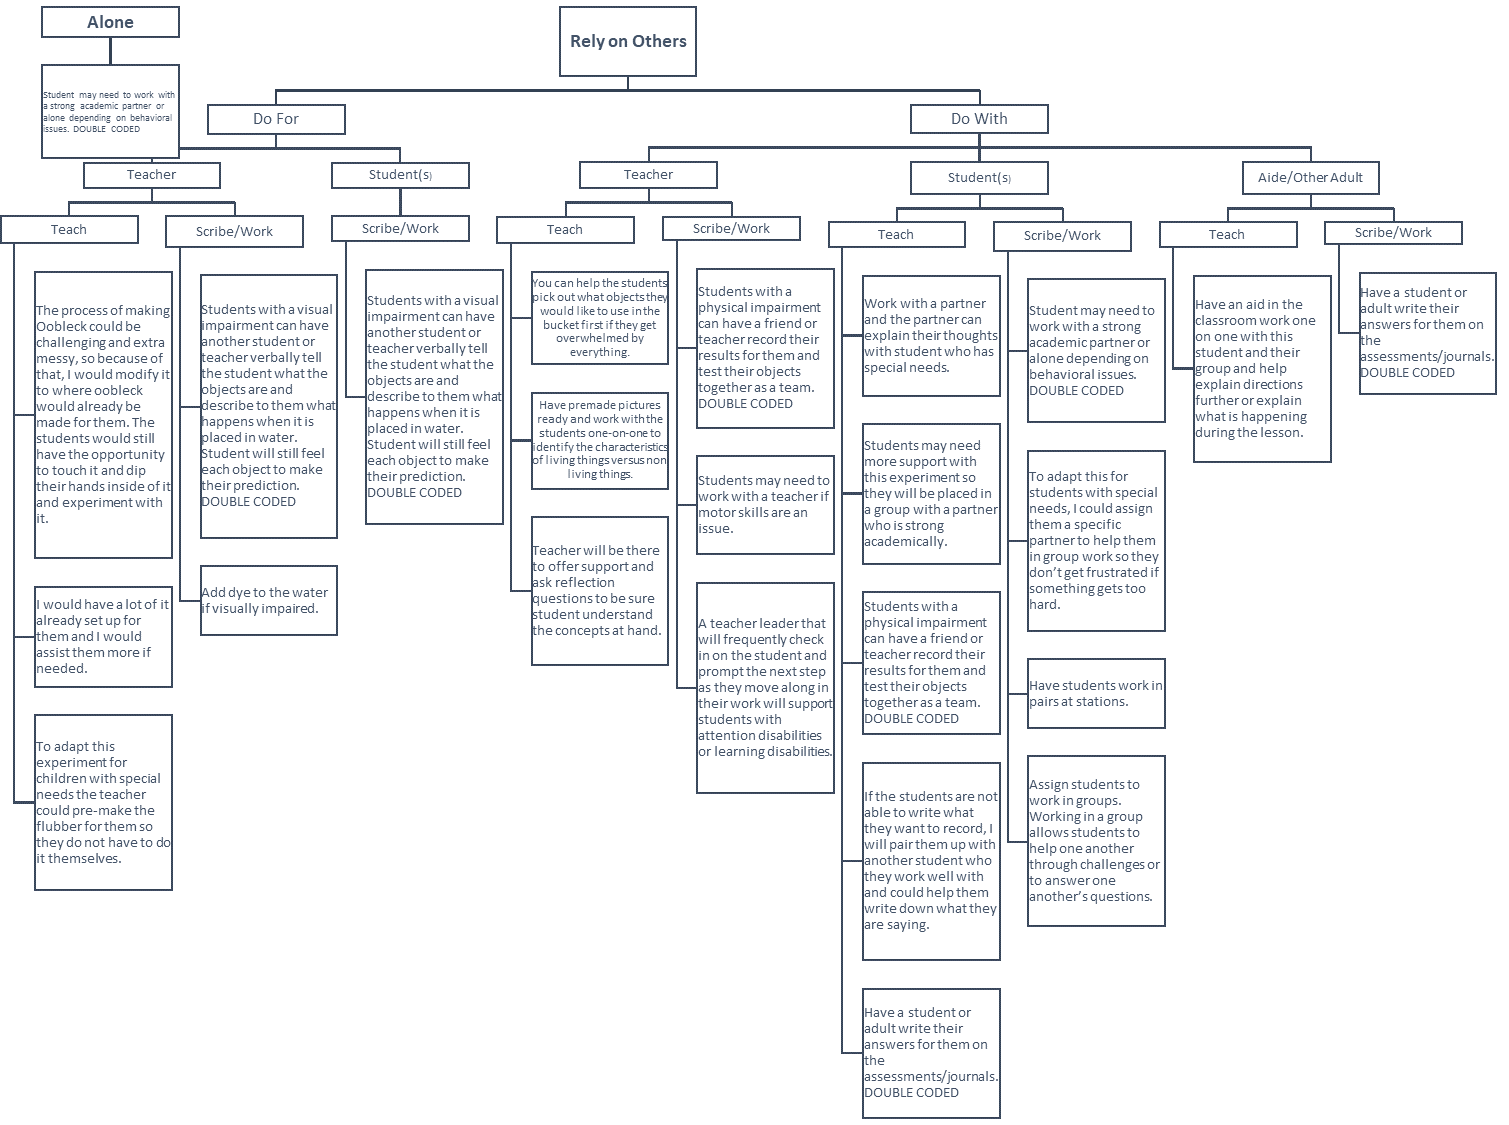
\includegraphics[width=1\textwidth]{Figure_2.png}
    \caption{Decision tree of “relying on others” as adaptation}
\end{figure*}

Given the focus on a variety of adaptations that can support students with disabilities, we were surprised by the paucity of meaningful adaptations that would enable students with a range of disabilities to participate fully in the inquiry-based science lessons.  Practices such as providing adaptive equipment (e.g., adaptive scissors, tactile meter sticks, magnifiers), advance organizers, pre-teaching vocabulary, and pictorial instructions, were all but absent from the lesson plans.  While use of UDL can reduce the need for such adaptations, it does not eliminate it.  We did not find that our teacher candidates exhausted means of reducing barriers for students before simply changing the lesson requirements.

We wonder if we contributed to this situation by not providing specific student case studies or other means of individualizing student needs for our teacher candidates.  By simply asking our teacher candidates for “Adaptations for Students with Disabilities,” our science lesson plan document may have unwittingly encouraged stereotyping and generalizations rather than prompting thoughtful, need-specific adaptations.  For our future lesson plan documents, we are considering asking teacher candidates to develop adaptations for two or three students in their own clinical field experiences (in addition to describing students’ strengths and challenges), or providing teacher candidates with case studies of specific students and eliciting their strategies for adaptations (McGinnis, 2003).  This revision may also help us as teacher educators to better understand the strong behavioral-influenced language in the late semester plans, which may have been inspired by particular experiences in teacher candidates’ field placement experiences, their methods instruction, or both.  We also wonder whether moving the prompt for accommodations for students with disabilities from the end of the lesson plan template to the beginning will promote greater use of UDL principles and more comprehensive, inclusive planning. 

Clearly, more work is needed to help teacher candidates recognize the continuum of adaptations that are available before they reduce expectations of their students with disabilities by either changing lesson objectives or having others do various aspects of the activities for them.  Resources such as the National Science Teachers Association’s web page on supporting students with disabilities in science (\url{http://www.nsta.org/disabilities/}) can be highlighted in both science and special education methods courses to provide teacher candidates with science-specific adaptations for all students. Researchers might also look to the use of high-leverage practices (McLeskey \& Brownell, 2015) for use in science classes.  These research-based practices represent those that are used frequently by special educators to increase achievement of a range of students across a wide variety of curriculum and perhaps most importantly for pre-service educators, are practices that can be mastered by novices.  Adapting these practices for science classrooms might be a useful step in ensuring that teacher candidates have a range of thoughtful, evidence-based practices from which to choose as they embark on the challenging and necessary work of ensuring that all students are included in high quality, inquiry-based science. 

\subsection*{Limitations and Future Research}

Several limitations must be considered when interpreting our results.  Because all of our participants were enrolled in both methods courses concurrently, we are unable to parse out the influences of the science methods vs. special education methods courses.  Future research using a quasi-experimental design would allow researchers to identify the relative contributions of the methods courses and topics.  In addition, we cannot quantify the effects of our teacher candidates’ mentor teachers, students within teacher candidates’ placement classrooms, and other “outside” influences. Social constructivism, when applied to teacher development, suggests that social interactions with others is a major factor in the construction of PCK (Bell 1998).  Future studies that triangulate data through the use of observations and interviews might mediate this limitation.  While our work focused on delivery of inclusive education through separate methods courses, research on the impacts of co-taught vs. separate methods courses on teacher candidate integration of inclusive science methods is also warranted.  Finally, given the different historical and philosophical influences between science and special education, it may be worth examining the best practices for balancing competing paradigmatic influences of explicit instruction vs. inquiry-based teaching to ensure that the goals of contemporary science education are met for all students. 

\end{large}
\clearpage{} 
\section*{REFERENCES}\par 

\leftskip 0.25in
\parindent -0.25in 
Ary, D., Jacobs, L.C., \& Sorensen, C. (2010). \textit{Introduction to research in education}.  Belmont, CA: Wadsworth.

Baglieri, S., Valle, J. W., Connor, D. J., \& Gallagher, D. J. (2011). Disability studies in education: The need for a plurality of perspectives on disability. \textit{Remedial and Special Education, 32}(4), 267-278. doi:10.1177/07419325103\\62200

Bell, B. (1998). Teacher development in science education. In B. J. Fraser \& K. G. Tobin (Eds.), \textit{International handbook of science education: Part two} (pp. 681–693). Dordrecht, The Netherlands: Kluwer.

Bybee, R. W., Taylor, J. A., Gardner, A., Van Scotter, P., Powell, J. C., Westbrook, A., \& Landes, N. (2006). \textit{The BSCS 5E instructional model: Origins and effectiveness}. Colorado Springs, Co: BSCS, 5, 88-98.

Cameron, D. L. \& Cook, B. G. (2007). Attitudes of preservice teachers enrolled in an infusion preparation program regarding planning and accommodations for included students with mental retardation. \textit{Education and Training in Developmental Disabilities, 42}, 353-63. Retrieved from \url{http://www.jstor.org/stable/23879628}

Government Accountability Office. (2009) Teacher Preparation: Multiple federal education offices support teacher preparation for instructing students with disabilities and English language learners, but systemic department wide coordination could enhance this assistance. (GAO Publication No. 09-573). Washington. D.C.: U.S. Government Printing Office. Retrieved from \url{http://www.gao.gov/assets/300/294208.pdf} 

Grossman, P.,  Hammerness, K.,  \& McDonald, M.  (2009) Redefining teaching, re‐imagining teacher education. \textit{Teachers and Teaching, 15}(2), 273-289. doi:10.1080/1354\\0600902875340

Individuals with Disabilities Education Act, 20 U.S.C. § 1400 (2004).

Irving, M., Nti, M., \& Johnson, W. (2007). Meeting the needs of the special learner in science. \textit{International Journal of Special Education, 22}(3), 109–118. Retrieved from \url{http://files.eric.ed.gov/fulltext/EJ814520.pdf}

Kahn, S., Feldman, A., Cooke, M. (2014). Signs of autonomy: Inquiry and autonomy in the deaf science classroom. \textit{Journal of Science Education for Students with Disabilities, 17}(1), 13-35. doi:10.14448/jsesd.06.0001

Kahn, S., \& Lewis, A. R. (2014). Survey on Teaching Science to K-12 Students with Disabilities: Teacher Preparedness and Attitudes. \textit{Journal of Science Teacher Education, 25}(8), 885-910. doi:10.1007/s10972-014-9406-z

Kellner, E., Gullberg, A., Attorps, I., Thorén, I., \& Tärneberg, R. (2011). Prospective teachers' initial conceptions about pupils' difficulties in science and mathematics: A potential resource in teacher education. \textit{International Journal of Science and Mathematics Education, 9}(4), 843-866. doi:10.1007/s10763-010-9232-5

King–Sears, M.E., Johnson, T.M., Berkeley, S., Weiss, M.P., Peters-Burton, E.E., Evmenova, A.S., … \& Hursh, J.C. (2015). An exploratory study of universal design for teaching chemistry to students with and without disabilities. \textit{Learning Disabilities Quarterly, 38}, 84-96. doi:10.1177/0731948714564575

Lincoln, Y.S. \& Guba, E.G. (1985). \textit{Naturalistic Inquiry}. Newbury Park, CA: Sage Publications.

Loughran, J., Milroy, P., Berry, A., Gunstone, R., \& Mulhall, P., (2001). Science cases in action: Documenting science teachers’ pedagogical content knowledge through PaP-eRs. \textit{Research in Science Education, 31}(2), 289-307. doi:10.1023/A:101312440

Mastropieri, M. A., Scruggs, T. E., Mantzicopoulos, P., Sturgeon, A., Goodwin, L., \& Chung, S. (1998). A place where living things affect and depend on each other: Qualitative and quantitative outcomes associated with inclusive science teaching. \textit{Science Education, 82}(2)163–179.

McCarthy, C. B. (2005). Effects of thematic-based, hands-on science teaching versus a textbook approach for students with disabilities. \textit{Journal of Research in Science Teaching, 42}(3)245–263. doi:10.1002/tea.20057

McLeskey, J., \& Brownell, M. (2015). High-leverage practices and teacher preparation in special education (Document No. PR-1). Retrieved from University of Florida, Collaboration for Effective Educator, Development, Accountability, and Reform Center website: \url{http://ceedar.education.ufl.edu/tools/best-practice-review/}

McGinnis, J. R. (2000). Teaching science as inquiry for students with disabilities. In J. Minstrell \& E. H. VanZee (Eds.), \textit{Inquiring into inquiry/learning and teaching in science} (pp.425-433). Washington, DC: American Association for the Advancement of Science. 

McGinnis, J. R. (2003). The morality of inclusive verses exclusive settings: Preparing teachers to teach students with mental disabilities in science. In D. Zeidler (Ed.), \textit{The role of moral	reasoning on socioscientific issues and discourse in science education} (pp. 196–215). 	Boston: Kluwer Academic Publishers.

McGinnis, J. R., \& Kahn, S. (2014). Special needs and talents in science learning. In N.G. Lederman \& S.K. Abell (Eds.), \textit{Handbook of research in science education} (Vol. II), (pp.223-245). New York, NY: Routledge.

Meyer, A., Rose, D., \& Gordon, D. (2014). \textit{Universal design for learning: Theory and practice}. Wakefield, MA: CAST Publications.

Miles, M. B., \& Huberman, A. M. (1994). \textit{Qualitative data analysis: An expanded sourcebook} (Second Ed.). Thousand Oaks, CA: Sage Publications.

Miller, B. (2012). Ensuring meaningful access to the science curriculum for students with significant cognitive disabilities. \textit{Teaching Exceptional Children, 44}(6), 16-25. doi:10.1177/004005991204400602

Moin, L.J., Magiera, K. \& Zigmond, N. (2009). Instructional activities and group work in the U.S. inclusive co-taught high school science class. \textit{International Journal of Science and Math Education, 7}(4) 677-697. doi:10.1007/s10763-008-9133-z

National Center for Education Statistics. (2011). The Nation’s Report Card: Science 2009 (NCES 2011-451). Washington, DC: Institute of Education Sciences, U.S. Department of Education.

National Center for Education Statistics. (2017). Children and Youth with Disabilities.	Washington, DC: Institute of Education Sciences, U.S. Department of Education. Retrieved from \url{https://nces.ed.gov/programs/coe/indicator\_cgg.asp}

National Council for Accreditation of Teacher Education. (2010). \textit{Transforming teacher education through clinical practice: A national strategy to prepare effective teachers}. Report of the Blue Ribbon Panel on Clinical Preparation and Partnerships for Improved Student Learning. Retrieved from \url{http://www.ncate.org/LinkClick.aspx?fileticket=zzeiB1OoqPk\%3D\&tabid=7}

National Education Technology Plan. (2016). \textit{Future ready learning: Reimagining the role of technology in education}. U.S. Department of Education: Office of Educational Technology Retrieved from \url{https://tech.ed.gov/files/2015/12/NETP16.pdf}

National Science Foundation, National Center for Science and Engineering Statistics. (2013). Women, minorities, and persons with disabilities in science and engineering: 2013. Special Report NSF13-304. Arlington, VA. Retrieved from	\url{http://www.nsf.gov/statistics/wmpd/}

Patton, M. Q. (2002). \textit{Qualitative research and evaluation methods} (3rd ed.). Thousand Oaks, CA: Sage.

Saldaña, J. (2016). \textit{The coding manual for qualitative researchers} (3rd ed.). London, UK: Sage.

Scruggs, T.E.,  \& Mastropieri, M.A. (2007). Science learning in special education: The case for constructed versus instructed learning. \textit{Exceptionality, 15}(2), 57-74. doi:10.1080/09362830701294144

Shulman, L.S. (1986). Those who understand: Knowledge growth in teaching. \textit{Educational Researcher, 17}(1), 4–14. doi:10.3102/0013189X015002004

Taylor, J.C., Therrien, W. J., Kaldenberg, E., Watt, S., Chanlen, N., \& Hand, B. (2012). Using an 	inquiry-based teaching approach to improve science outcomes for students with disabilities: snapshot and longitudinal data. \textit{Journal of Science Education for Students 	with Disabilities, 15}(1), 27-39. doi:10.14448/jsesd.04.0003

Therrien, W. J., Taylor, J. C., Hosp, J. L., Kaldenberg, E. R., \& Gorsh, J. (2011). Science instruction for students with learning disabilities: A meta-analysis. \textit{Learning Disabilities Research \& Practice, 26}(4), 188–203. doi:10.1111/j.1540-5826.2011.00340.x

Wild, T. A., \& Trundle, K. C. (2010). \textit{Conceptual understandings of seasonal change by middle school students with visual impairments. Journal of Visual Impairment \& Blindness, 104}(2), 107-118. Retrieved from \url{https://eric.ed.gov/?id=EJ874438}

\end{document}